\chapter{Detecção de eventos através do Twitter}

O Twitter possui um imenso banco de dados de publicações criadas por usuários, tornando-se uma fonte para aplicação de técnicas de análise de texto. Além do texto propriamente dito de cada publicação, o serviço também armazena dados úteis como o horário em que a ela foi criada e a localização do usuário ao criá-la.

O serviço disponiliza as informações das publicações através de interfaces de aplicação, para que aplicações externas possam realizar buscas de forma automatizada, além de outras ações. O modelo de detector de eventos proposto utiliza as publicações disponibilizadas pelo Twitter como fonte de dados para detectar ocorrências de manifestações. O detector se apoia nas informações criadas por seus usuários para retirar informações relevantes como o local e o horário de manifestações.

Para validar o detector de eventos proposto, o modelo busca por publicações que contém a palavra-chave ``manifestação'', criadas no mês de Agosto de 2014. Todas as publicações contendo a palavra-chave são copiadas para um ambiente de trabalho local. 

As publicações obtidas, porém, não passam por filtros ao serem criadas e diversas delas devem ser descartadas para o processo de detecção. Mesmo contendo a palavra-chave buscada, muitas podem não dizer respeito ao evento que o modelo deseja detectar. Para classificar as publicações que são relevantes para o modelo e as que devem ser descartadas, o modelo utiliza a técnica de aprendizado de máquina SVM como \textit{classificador de texto}. 

O SVM é um método de aprendizado supervisionado em que, através de um conjunto inicial de exemplos previamente classificados, consegue induzir em qual classe uma nova ocorrência se encaixa. O modelo utiliza um conjunto de \textit{publicações de treino}, previamente classificadas entre ocorrências positivas, ou seja, indicam a ocorrência real de um evento de manifestação, e negativas, não indicam a ocorrência, podendo ser apenas o termo empregado em outro contexto, ser referente à uma manifestação futura ou passada, etc. Esse processo é chamado de \textit{representação do conhecimento}, que é quando o conhecimento do ambiente (publicações sobre manifestações) é passado para a máquina de aprendizado, que analisa os padrões das informações e adquire o conhecimento.

Com o conhecimento representado, o SVM pode classificar novas ocorrências. Porém, o SVM não recebe como entrada o texto das publicações, e sim a sua representação matemática. O modelo implementado representa os textos no \textit{modelo de espaço vetorial}, aonde eles são convertidos para um vetor que contem as informações relacionadas à presença ou ausência de seus termos. Para converter, as publicações são divididas em termos, separados por espaço, e é criado um dicionário dos termos de todas as publicações. Através dessa representação, o SVM realiza operações matemáticas que determinam as relações de distância entre os dados, podendo inferir à qual classificação cada dado se enquadra.

Após a classificação das publicações, o modelo extrai o horário e a localização das publicações positivas. A informação do horário será utilizada para agrupar as publicações, com o intuito de determinar os horários em que ocorreram mais ocorrências de menções à manifestações. Os horários de pico representam os \textit{eventos}, que são ocorrências anômalas ao funcionamento normal do fluxo contínuo de publicações. Já a localização será utilizada para a analise visual das regiões de ocorrência dos eventos, que serão traçadas nos mapas apresentados. A arquitetura proposta é ilustrada na Figura 3.1.

\section{Publicações como fonte de dados}

No Twitter, cerca de 500 milhões de publicações\footnote{http://www.internetlivestats.com/twitter-statistics/} são criadas diariamente, e junto com elas, diversos dados úteis são gravados. Uma publicação é o conjunto de dados de uma mensagem que é enviada ao servidor do Twitter. Cada texto de uma publicação é limitado a 140 caracteres, e possui também dados adicionais como:

\begin{itemize}
	\item Horário de criação
	\item Idioma
	\item Dados do usuário que a publicou como nome, localização, descrição e foto
	\item Geolocalização (para envios de smartphones, tablets e notebooks com essa opção ativada)
	\item Referências à links, usuários e hashtags, caso possuam
	\item Publicação na qual está respondendo 
\end{itemize}

\begin{figure}[htpb]
\begin{center}
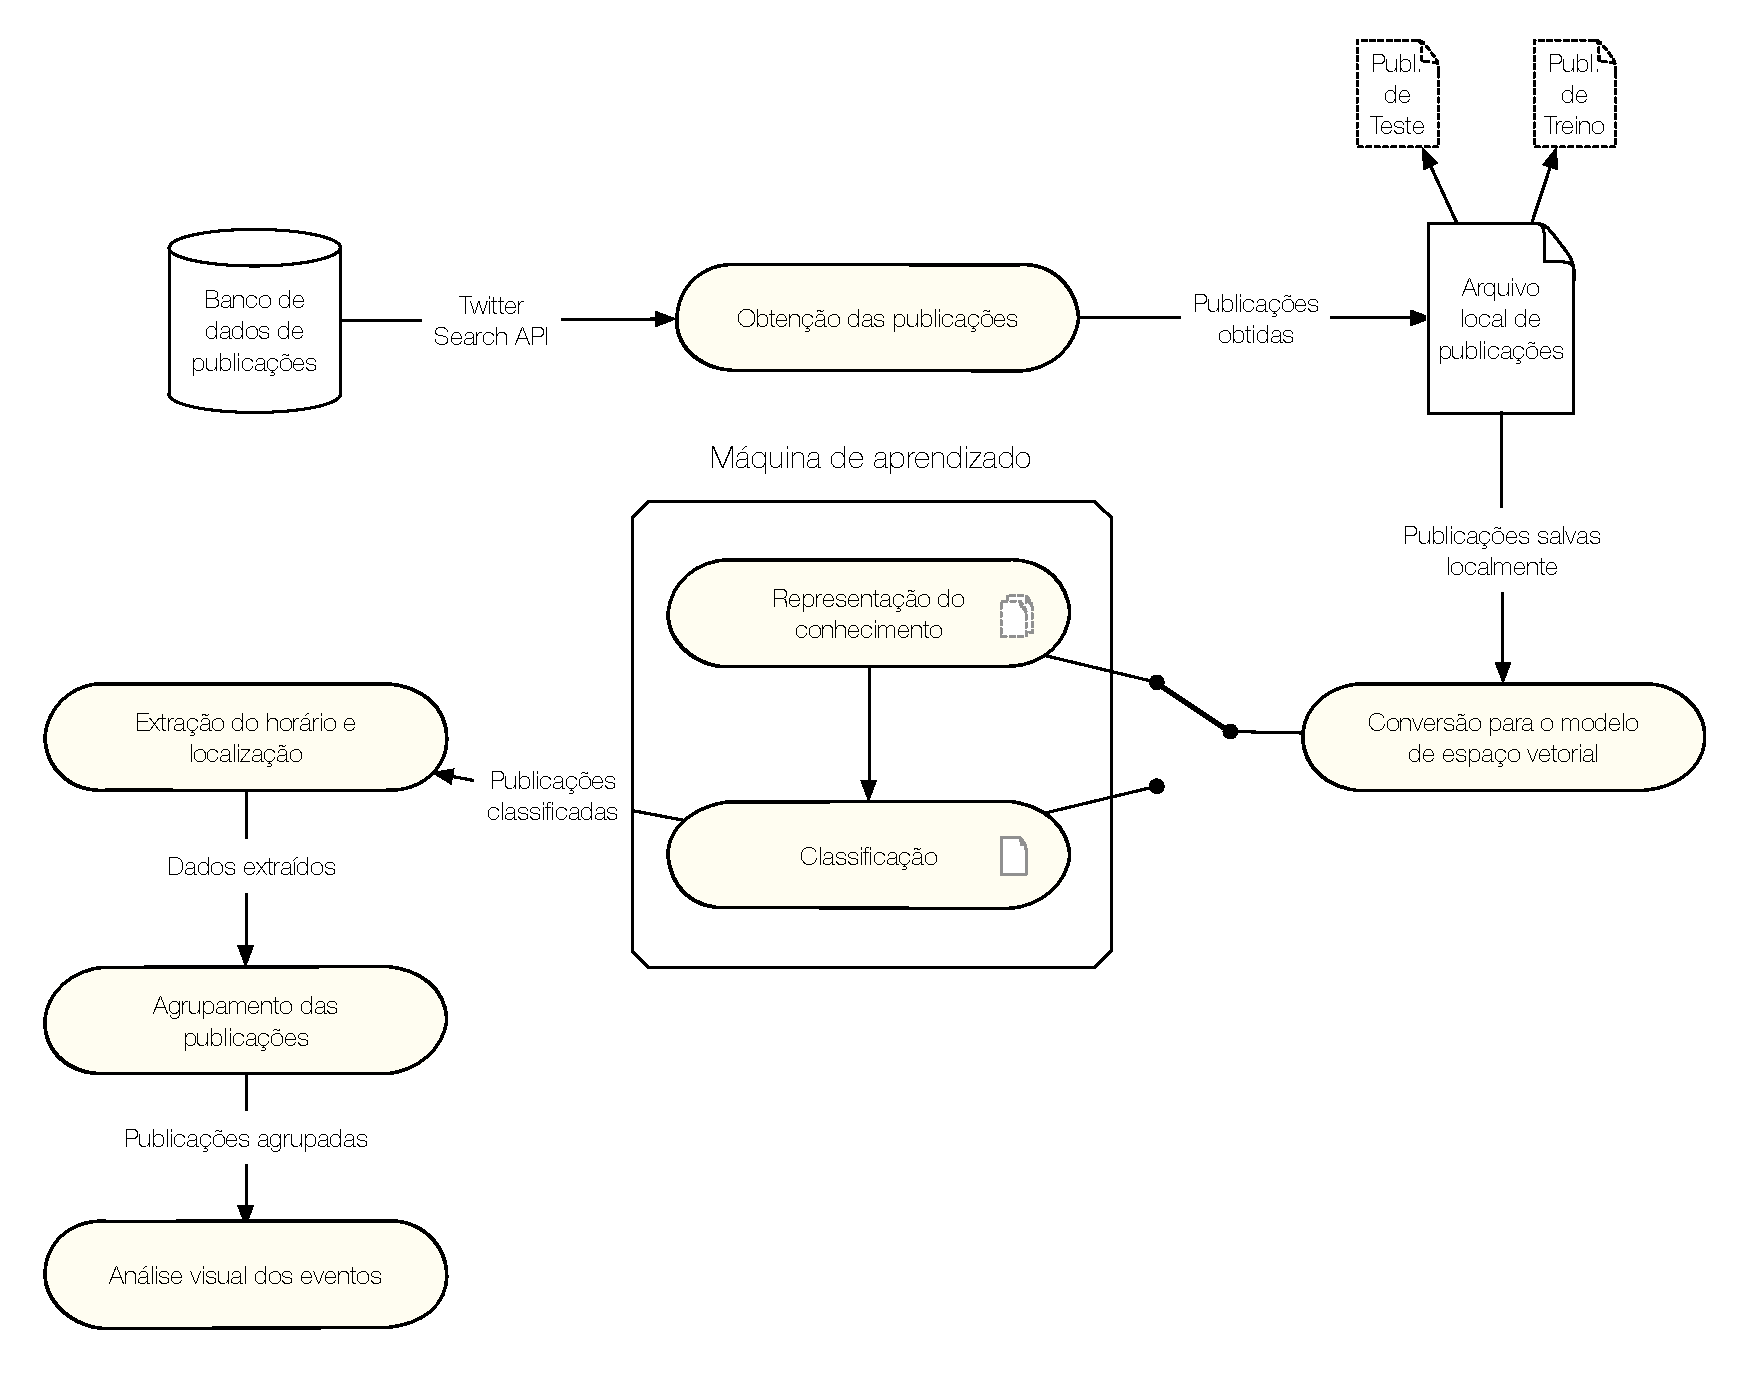
\includegraphics[width=1.0\textwidth]{figuras/fluxograma-deteccao.eps}
\caption{Processo de detecção para o detector de eventos proposto.}
\end{center}
\end{figure}

As publicações são criadas por usuários e dizem respeito aos mais variados eventos dos mundo real. Com o acesso à essas publicações é possível melhorar serviços externos, prever resultados de votações, monitorar opiniões sobre marcas, detectar desastres naturais etc. \citeonline{Tumasjan2010}, por exemplo, acham um grande paralelo entre o sentimento político dentro das publicações no serviço e fora do mesmo. \citeonline{Stankovic2010} criam uma ferramenta que mapeia as publicações que são referentes à conferências. Já \citeonline{Cox2011} utilizam as publicações referentes à observações sobre o clima para melhorar as previsões do tempo.

As publicações, por serem criadas por usuários, não passam por qualquer tipo de filtro, e grande parte delas devem ser descartadas para o sucesso das análises, seja por conter palavras com a grafia errada, gírias, ou por não dizerem respeito à qualquer conteúdo relevante. De acordo com a \citeonline{PearAnalytics2009}, aproximadamente 40\% das publicações não possuem relevância, atuando apenas como ruído para as análises.

Para o sucesso das técnicas de análise que utilizam publicações como dados de entrada, é necessário que o processo reconheça adequadamente as publicações que são apenas ruídos e as tratem, processem e/ou excluam, para que os resultados obtidos sejam relevantes e satisfatórios.

Na detecção de eventos, é preciso também que o evento contenha quantidade suficiente de publicações relacionadas. Apenas eventos com certa relevância podem ser detectados, pois caso contrário não haverá quantidade suficiente de publicações para gerar análises consistentes. Segundo \citeonline{Sakaki2010}, alguns fatores, como escala, influência e região, aumentam a probabilidade que um evento possa ser detectado no Twitter.

\begin{itemize}
	\item \textbf{Escala:} Eventos com grande escala são vivenciados por muitas pessoas, gerando uma maior quantidade de publicações.
	\item \textbf{Influência:} Eventos com maior grau de influência na vida dos pessoas tendem induzi-las mais a compartilhar a experiência e gerar publicações.
	\item \textbf{Região:} Eventos com região de espaço e tempo delimitados permitem que sejam feitas estimativas do horário e da localização.
\end{itemize}

Eventos de grande escala, com alto grau de influência e com região de tempo e espaço são os tipos de eventos mais propícios para a aplicação da detecção de eventos, pois geram um maior fluxo de publicações e permitem a estimativa da sua localização. Alguns exemplos de eventos com essas características são desastres naturais como terremotos, tempestades, ciclones e tufões, eventos sociais como grandes festivais, eventos esportivos e políticos e desastres não naturais como acidentes de todos os tipos.

A obtenção das publicacões é feita através das \textit{interfaces de aplicação} do Twitter, que disponibilizam seus dados através de uma formatação em texto estruturada.

\section{Interfaces para obtenção dos dados}

Para disponibilizar as publicações, o serviço utiliza a forma de notação JSON (\textit{JavaScript Object Notation}) para troca de dados. Uma formatação leve, em formato de texto, que permite que os dados das publicações sejam transferidos pela rede de internet para serviços externos. Os dados são estruturados em pares de nome/valor e possuem ordem fixa. O Código 3.1 apresenta a estrutura da uma publicação, com dados como data de criação, id, texto, etc.

\begin{lstlisting}[caption=Estrutura JSON de uma publicação]
	{
		:created_at=>"Thu Jul 31 15:14:27 +0000 2014",
	  :id=>494863667100258304,
    :text=>"Manifestacao deixa transito congestionado em Sao Cristovao: Funcionarios do transporte alternativo protestam...",
	  (...)
    :user=>{
    	:id=>2340427167,	
      :name=>"Rodrigo",
      :location=>"Sao Paulo",
      (...)
     },
    :geo=>nil,
    :coordinates=>nil,
    :place=>nil,
    (...),
    :lang=>"pt"
  }
\end{lstlisting}

Para transferir os dados, o Twitter disponibiliza interfaces de aplicação (APIs: \textit{Application Product Interfaces}) poderosas que permitem com que os desenvolvedores utilizem as informações disponíveis em seu serviço para os mais variados fins. São elas: \textit{Search API}, \textit{REST API} e \textit{Streaming API}\footnote{https://dev.twitter.com/start}.

\subsection*{REST API}

A \textit{REST API} é a interface mais básica do Twitter, que permite que desenvolvedores acessem as principais ações do serviço, como informações de usuários, atualizações de status e menções à um usuário específico. Além de permitir a criação de publicações, a resposta à outras publicações, o \textit{retweet} e que usuários as favoritem através de serviços externos. 

Uma das formas de utilizar a \textit{REST API} constitui em criar um servidor HTTP mediador das ações entre o usuário e o Twitter. O servidor recebe as ações do usuário em seu website, analisa a requisição e então a repassa para o Twitter para realizar qualquer ação necessária para enviar a resposta para o usuário. O website então atualiza sua página e o usuário vê as informações que pediu, como segue na Figura 3.2.

\begin{figure}[htpb]
	\begin{center}
	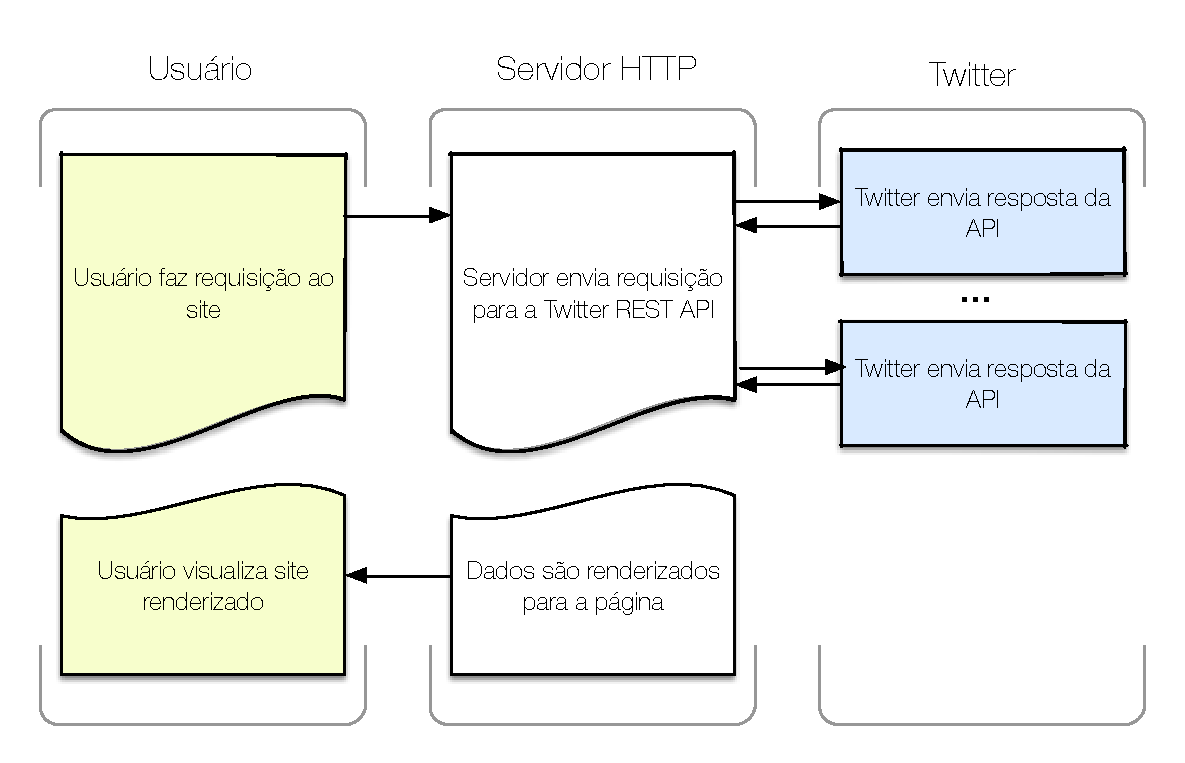
\includegraphics[width=0.8\textwidth]{figuras/twitter-rest-api.eps}
	\caption{Funcionamento da REST API do Twitter.}
	\end{center}
\end{figure}

\subsection*{Search API}

A \textit{Search API} faz parte da \textit{REST API} e é a interface do Twitter que serve com o propósito específico de buscar por publicações. Ela permite que desenvolvedores façam buscas por publicacões através de palavras-chave específicas, além de forneceder operadores para que a busca seja refinada. 

A \textit{Search API} é focada na relevância dos dados, não em sua totalidade, ou seja, apenas as publicações serão retornadas e existe um limite de resultados à serem retornados. Na Tabela 3.1 estão representados alguns dos operadores disponíveis.

\begin{table}[ht]
	\caption{Operadores da Search API}
	\centering
	\begin{tabular}{| l | l |}
		\hline
		\textbf{Operador} & \textbf{Busca por publicações contendo...} \\ [0.5ex] \hline \hline
    assistindo agora & contendo ``assistindo'' e ``agora'' \\
    ``chegando em casa'' & contendo exatamente a frase ``chegando em casa'' \\
    amor OR ódio & contendo ``amor'' ou ``ódio'' (ou os dois) \\
    amor -ódio & contendo ``amor'' mas não ``ódio'' \\
    \#copa & contendo a hashtag ``copa'' \\
    @mashable & referenciando o usuário ``mashable''  \\ 
    ... & ... \\ [1ex]
		\hline
	\end{tabular}
	\label{table:nonlin}
\end{table}

Por exemplo, buscando pelo termo ``estou aqui'', o serviço retorna todas as publicações com os termos ``estou'' e ``aqui'', independente da ordem e da posição das palavras na mensagem. Ao buscar pelos termos entre aspas, o serviço retorna as publicações contendo exatamente a expressão pesquisada. Existe também o operador lógico ``OR'', que retorna as publicações que contem uma palvavra ou a outra. Além da busca por \textit{hashtags} (\#) e menções aos usuários (@). Essas, porém, não constituem todas as buscas possíveis no serviço, sendo possível inclusive combinar os operadores\footnote{https://dev.twitter.com/docs/using-search}.

\subsection*{Streaming API}

A \textit{Streaming API} é a interface do Twitter que permite acesso de baixa latência e sem os limites da \textit{Search API}. Com ela, é possível fazer requisições em tempo real para o serviço, obtendo as publicações conforme são criadas.

Nessa API, o primeiro passo é solicitar uma conexão permanente (streaming) com o servidor do Twitter, que então aceita a sua solicitação e abre a conexão. O Twitter começa, então, a enviar as publicações de forma automática, conforme elas são criadas. O serviço que solicitou se encarrega de processá-las e guardá-las como for conveniente. O usuário então, ao acessar o serviço, faz a requisão e o serviço obtém os dados processados de seu banco de dados (não diretamente do Twitter) e renderiza a página para que o usuário possa visualizar os resultados, como explicitado na Figura 3.3.

\begin{figure}[htpb]
\begin{center}
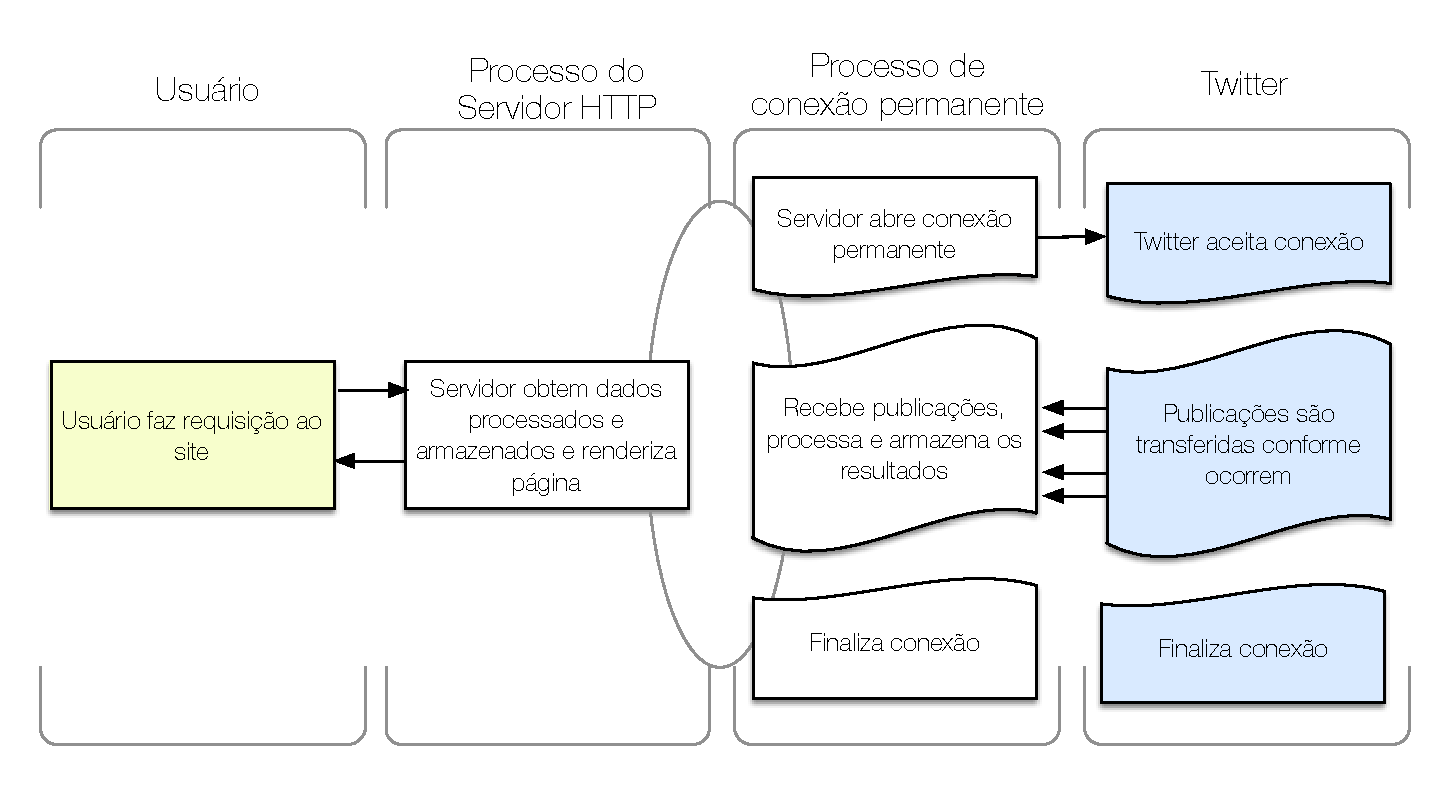
\includegraphics[width=1.0\textwidth]{figuras/twitter-streaming-api.eps}
\caption{Funcionamento da Streaming API do Twitter.}
\end{center}
\end{figure}

A elipse central da Figura 3.3 representa que os dois lados estão conectados, mas não de forma síncrona. Para o \textit{servidor HTTP} obter os dados processados, é necessário que, antes a \textit{conexão permamente} tenha sido criada e as publicações obtidas. Porém, o intervalo entre a obtenção das publicações e a requisição do usuário pode ser variado. É possível que a \textit{conexão permanente} já tenha sido terminada antes da requisição para o \textit{servidor HTTP}, ou também que os dois estejam agindo simultaneamente.

\section{Obtenção dos dados}

A primeira etapa para a implementação de um detector de eventos é a obtenção dos dados. Para o modelo implementado, os dados são obtidos do banco de dados do Twitter, através de sua interface para desenvolvedores. A interface permite que a informação trafegue pela rede através do formato de texto. Com a busca por uma palavra-chave específica, o serviço reune todas as publicações referentes à ela em um arquivo de texto e o envia de forma estruturada, para que localmente esses dados sejam tratados e salvos de várias maneiras.

O modelo utiliza a interface \textit{Search API} para buscar por publicações. Como o serviço informa, essa interface não disponibiliza a quantidade total de publicações criadas, e sim as mais relevantes - para ter acesso à todas as publicações é necessário utilizar a \textit{Streaming API}. Por isso, foram realizados testes para definir se a interface servia para o propósito do modelo. 

Os testes mostraram que a \textit{Search API} retorna quantidade relevante de publicações e elimina a necessidade da implementação de um servidor com conexão permanente com o Twitter, o que seria necessário para a utilização da \textit{Streaming API}. Caso o servidor caísse, seriam perdidas as publicações criadas nesse período, e não seria possível a busca por publicações anterior ao período de criação do servidor.

Para validar o modelo implementado, pretende-se detectar ocorrências de manifestações no território brasileiro no mês de Agosto de 2014. Para isso, é realizada a busca por publicações com a palavra-chave ``manifestação''. 

Como a interface utilizada retorna apenas publicações criadas há, no máximo, uma semana, torna-se necessário programar mais de uma busca, em diferentes datas. Após a obtenção dos dados estruturados das publicações em formato JSON, são selecionados os seguintes dados: 

\begin{itemize}
	\item Texto da publicação
	\item Horário de criação da publicação
	\item Latitude e longitude do usuário
	\item Localização configurada perfil do usuário
	\item Identificador único da publicação
\end{itemize}

O texto da publicação é a publicação propriamente dita, que serve com o propósito de detectar as ocorrências de manifestação. O horário de criação, a latitude e longitude e a localização configurada no perfil são utilizadas em passos posteriores para o agrupamento das publicações. O identificador único é útil para definir a última publicação buscada e definir, na próxima busca, em qual publicação a busca irá parar.

Os dados selecionados são gravados localmente em um arquivo CSV (\textit{comma separated values}), um formato de dados em texto em que os campos são separados por vírgulas. Os dados formam uma tabela, sendo as vírgulas delimitadoras das colunas e as quebra de linha delimitadoras de linhas. São adicionadas aspas nos campos para impedir que as vírgulas dos textos se confundam com as vírgulas separadoras dos campos. A Tabela 3.2 representa exemplos de publicações contidas no arquivo CSV.

\begin{table}[ht]
	\caption{Representação em tabela do arquivo CSV}
	\centering
	\begin{tabular}{| p{1cm} | p{2cm} | p{4cm} | p{2cm} | p{2cm} | p{2.5cm} |}
		\hline
		\textbf{Id} & \textbf{Horário} & \textbf{Texto} & \textbf{Latitude} &\textbf{Longitude} & \textbf{Localização perfil} \\ [0.5ex] \hline \hline
    49744 40914 21286 400 & 2014-08-07 14:45:23 & Aumento da passagem de ônibus provoca manifestação em sorocaba & -15.850902 & -47.944792 & Brazil \\ \hline
    49743 91868 07685 121 & 2014-08-07 14:40:19 & Grupo faz manifestação contra assassinatos de mulheres em goiânia &  &  &  \\ \hline
    49743 54381 48104 192 & 2014-08-07 14:39:50 & sabe se já acabou a manifestação??? &  &  & Rio de Janeiro - Brasil \\
    ... & ... & ... & ... & ... & ... \\
		\hline
	\end{tabular}
	\label{table:nonlin}
\end{table}

Com as publicações gravadas no arquivo CSV, são selecionadas algumas publicações para gerar dois outros arquivos: um que irá conter as \textit{publicações de treino} e outro que irá conter as \textit{publicações de teste}. Os novos arquivos terão o propósito de fornecer as publicações para representar o conhecimento para o SVM.

Após a obtenção das publicações, então, cada uma é convertida para o seu modelo de espaço vetorial, para que o SVM utilize a representação vetorial de cada publicação e possa classificá-las de acordo com suas características.

\section{Modelo de espaço vetorial}

O \textit{modelo de espaço vetorial} é um modelo de representação de dados em vetores de características. Os vetores são constituídos por termos de índice, que podem conter pesos de acordo com sua importância ou não \cite{Salton1975}. Os vetores são utilizados para analises estruturas e operações matemáticas a partir dos dados convertidos, o que não seria possível a partir dos dados originais, como documentos de texto. 

Para a conversão de dados para o modelo de espaço vetorial, são escolhidos em quais tipos de recursos ele é constituído. Os recursos, em documentos texto, podem ser um conjunto de termos separados por espaço, frases separadas por pontuação, quebra de linha, etc. Segundo \citeonline{Joachims1998}, os recursos provenientes de documentos de texto possuem as seguintes características:

\begin{itemize}
	\item \textbf{Alta dimensão:} Os recursos geralmente são as palavras presentes nos documentos, ou seja, podem chegar à altíssimas dimensões, uma vez que cada palavra será uma dimensão no vetor de recursos.
	\item \textbf{Poucos recursos irrelevantes:} Nos documentos de texto, poucos recursos são irrelevantes, mantendo a sua alta dimensão e impedindo que algoritmos classificadores baseados na remoção de recursos irrelevantes sejam utilizados.
	\item \textbf{Dados esparsos:} Para cada documento, o vetor de características correspondente contém apenas algumas entradas que não são zero, pois possui apenas alguns dos termos do dicionário.
\end{itemize}

O recurso escolhido pelo modelo implementado é a presênca ou ausência de palavras em cada publicação. Palavras são todas os conjuntos de caracteres separados por espaço, o que chamamos de \textit{termo}. Primeiramente, aplica-se a \textit{tokenização} nas publicações, para gerar os seus termos constituintes. Os termos passam, então, pelo \textit{pré-processamento}, que agrupa termos que possuem o mesmo significado, como palavras seguidas de pontuação e maiúsculas ou minúsculas. 

Todos os termos são então agrupados e ordenados em ordem alfabética, criando assim o \textit{dicionário de termos}. No dicionário, cada termo possui um identificador único, idêntico à sua ordem. Após a criação do dicionário, cada publicação é convertida para sua representação no modelo de espaço vetorial, aonde os seus vetores de características são extraídos de acordo com os termos presentes e o índice desses termos no dicionário. Na Figura 3.4 estão apresentadas as fases da conversão para o modelo de espaço vetorial.

\begin{figure}[htpb]
	\begin{center}
		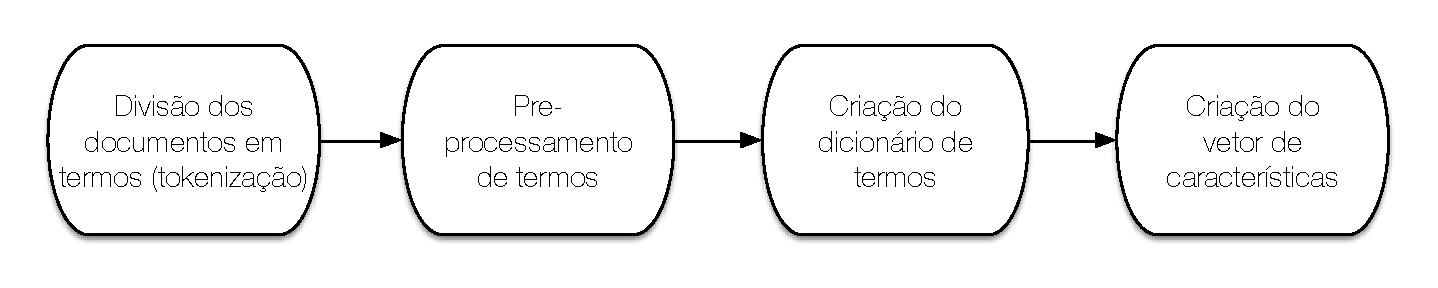
\includegraphics[width=1.0\textwidth]{figuras/processo-modelo-espaco-vetorial.eps}
		\caption{Processo de conversão para o modelo de espaço vetorial.}
	\end{center}
\end{figure}

\subsection{Tokenização}

A tokenização é o primeiro passo na conversão para o modelo de espaço vetorial, nela os documentos são convertidos em um conjunto de termos. Os delimitadores de termos podem ser espaços, pontuação, linhas, etc. Alguns processos de tokenização, pode ser mais complexos do que isso, por exemplo, como indicado por \citeonline{Turney2010}, alguns \textit{tokenizadores} devem ser capazes de reconhecer termos de mais de uma palavra, como ``Barack Obama'', termos que contém hífem e pontuação, ignorar pronomes e preposições, etc.

O modelo implementado utiliza espaços para delimitar os termos de cada publicação e utiliza uma lista de palavras muito recorrentes, como preposições, para ignorá-las na criação dos termos, como ``em'', ``no'', ``de'', etc. Links também não geram termos, ou seja, todos os termos que começam com ``http://'' são ignorados.

O processo de tokenização divide a publicação em um vetor de $n$ termos. Por exemplo, a publicação ``Manifestação em Goiânia!'' é transformada no conjunto de 3 termos: ``Manifestação'', ``em'', ``Goiânia!'', como indicado na Figura 3.5.

\begin{figure}[htpb]
	\begin{center}
		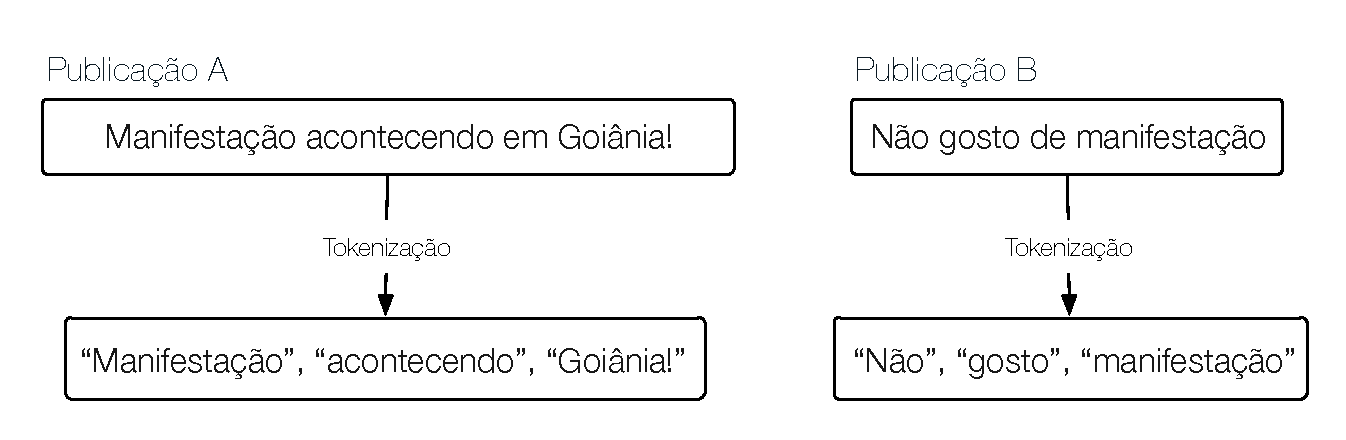
\includegraphics[width=1.0\textwidth]{figuras/tokenizacao.eps}
		\caption{Tokenização de duas publicações.}
	\end{center}
\end{figure}

A tokenização, porém, não trata de casos como o do termo ``Goiânia!''. Nesse caso, somente a pontuação e a letra maiúscula faz com que um novo termo seja criado, diferenciando-o de ``Goiânia'' e ``goiânia'', por exemplo. Isso adiciona complexidade à classificação, pois quanto mais termos, maior a dimensão dos dados a serem analisados. Para tratar desses casos, é necessário o \textit{pré-processamento} dos termos.

\subsection{Pré-processamento}

O pré-processamento é encarregado de normalizar os termos, para que não haja diferenciação entre termos que são essencialmente iguais. Isso diminui a complexidade da análise dos dados, na medida em que reduz a dimensão dos vetores de características.

No modelo implementado, os termos são pré-processados removendo suas pontuações e transformando-os para minúsculas. Ou seja, o pré-processamento retira a diferenciação de termos como ``manifestação'', ``Manifestação'' e ``manifestação.''. Todos os exemplos, após o pré-processamento, são identificados como o mesmo termo. Na Figura 3.6 é demonstrado o pré-processamento para duas publicações.

\begin{figure}[htpb]
	\begin{center}
		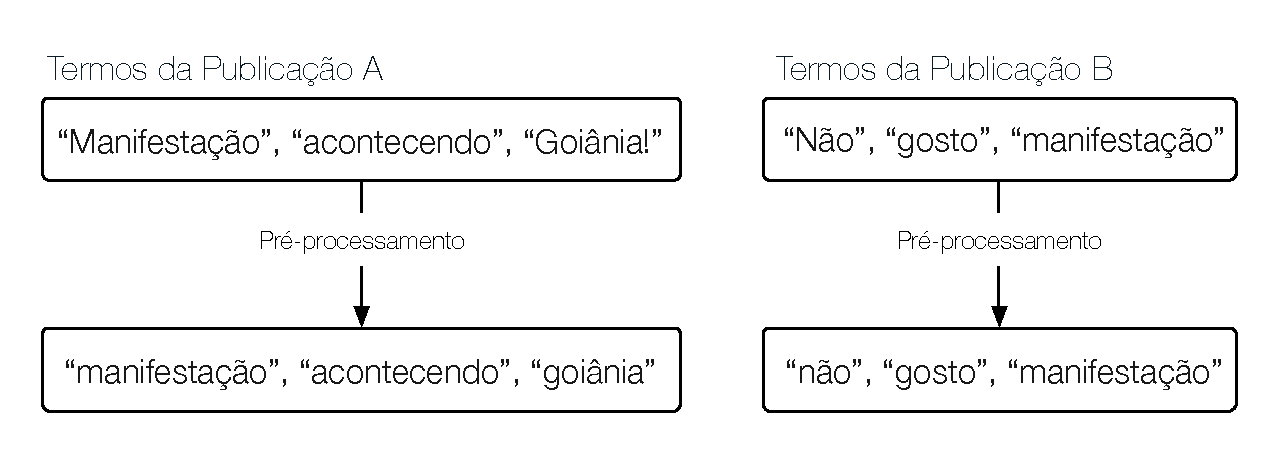
\includegraphics[width=1.0\textwidth]{figuras/pre-processamento.eps}
		\caption{Pré-processamento de duas publicações.}
	\end{center}
\end{figure}

\subsection{Criação do dicionário de termos}

Após pré-processados os termos, é criado um dicionário de todos os termos obtidos, o \textit{dicionário de termos}. No dicionário, os termos são únicos, não importando quantas vezes são repetidos no conjunto de publicações. Os termos são também ordenados em ordem alfabética, o que concede um identificador único para cada termo. O primeiro termo possui identificador ``0'', o segundo ``1'', e assim por diante.

A quantidade de termos do dicionário define a dimensão dos vetores de caraterísticas das publicações. Todos os vetores terão a dimensão da quantidade de termos no dicionário, e cada elemento do vetor representa um termo do dicionário. O primeiro elemento de cada vetor será referente ao primeiro termo do dicionário, e seu valor depende se a publicação contém o termo ou não. A Figura 3.7 representa um dicionário para duas publicações.

\begin{figure}[htpb]
	\begin{center}
		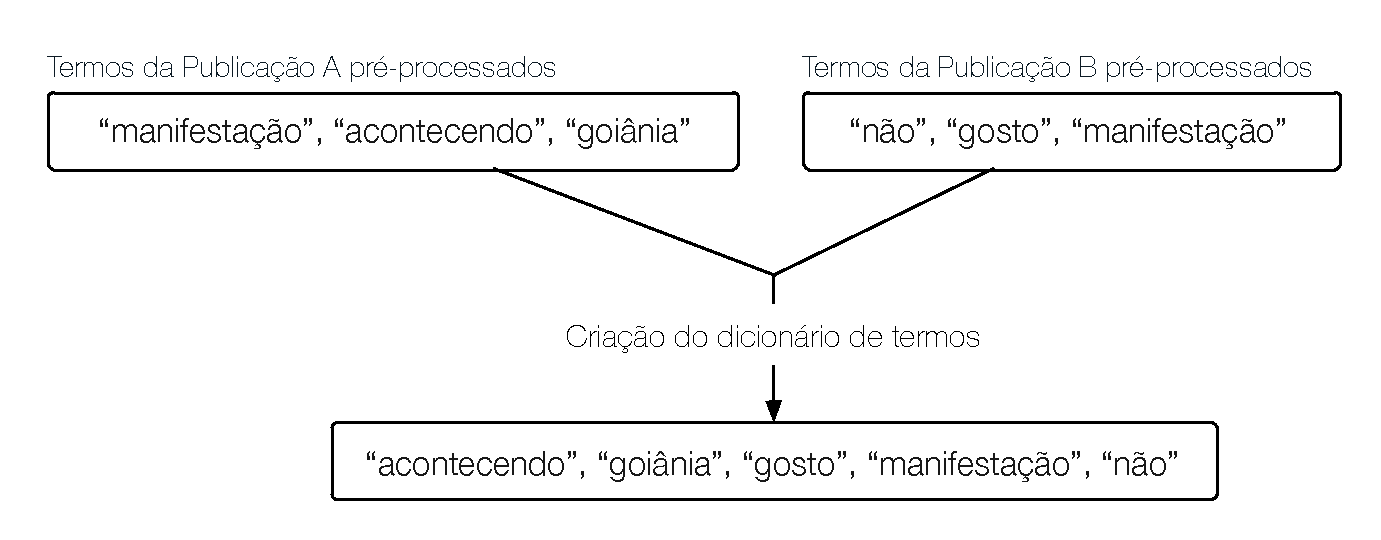
\includegraphics[width=1.0\textwidth]{figuras/dicionario-termos.eps}
		\caption{Dicionário de termos de duas publicações.}
	\end{center}
\end{figure}

\subsection{Criação do vetor de características}

À partir do dicionário, é possível a extração do vetor de características de cada publicação. O valor de cada elemento do vetor será ``1'' se a publicação contém o termo, ou ``0'' se a publicação não contém. Ou seja, se o primeiro termo do dicionário é a palavra ``gosto'', e o vetor é referente à publicação ``não gosto de manifestação'', a sua primeira posição será o valor ``1'', pois a publicação contém termo ``gosto''. Se o segundo termo for ``rua'', a segunda posição do vetor dessa publicação possuirá o valor ``0'', pois não possui o termo, e assim por diante. A Figura 3.8 representa a criação do vetor de características para duas publicações.

\begin{figure}[htpb]
	\begin{center}
		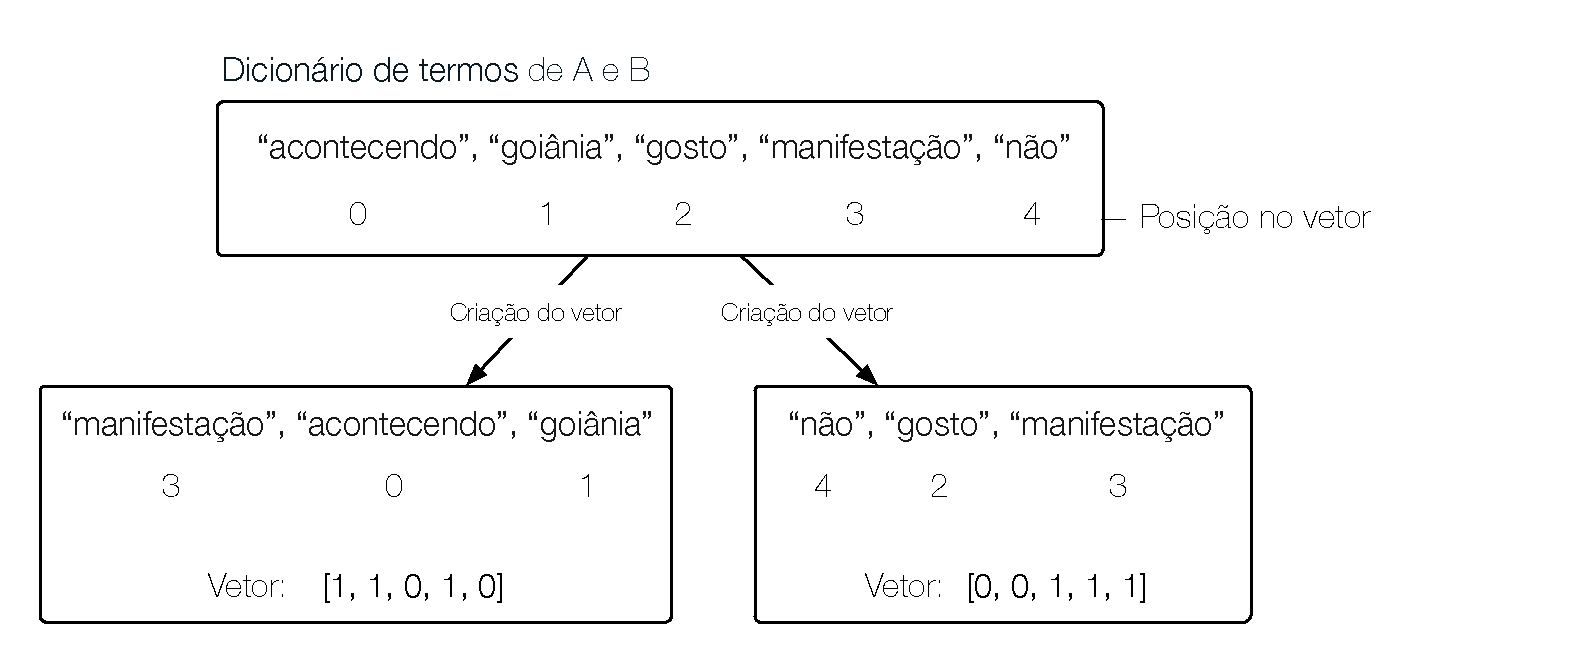
\includegraphics[width=1.0\textwidth]{figuras/vetor-caracteristicas.eps}
		\caption{Criação do modelo de características de duas publicações.}
	\end{center}
\end{figure}

A \textit{Publicação A} é representada pelo vetor [1, 1, 0, 1, 0] - os índices 0, 1 e 3 são marcados como ``1'' pois possuem os termos respectivos no dicionário, e os índices 2, 4 como ``0'' pois não possuem. Similarmente, a \textit{Publicação B} é representada pelo vetor [0, 0, 1, 1, 1].

A conversão dos documentos é necessária para que a classificação das publicações ocorra, pois o classificador não análisa os documentos no formato de texto, e sim na forma de vetores no modelo de espaço vetorial. Cada publicação no modelo de espaço vetorial será um vetor de alta dimensão e muito esparso, ou seja, conterá muitos ``0'', porém a técnica utilizada para classificação posterior é conhecida por ser capaz de lidar com dados com essas características.

\section{Extração dos dados}

A extração e o agrupamento dos dados da publicação, como horário e localização, são relevantes para a sua demonstração no ambiente interativo. Para extrair o \textit{horário} de um evento, o modelo utiliza apenas informação contida na estrutura da publicação. Para extrair a \textit{localização}, são utilizadas três fontes de dados, na ordem: a geolocalização, a cidade na definição do perfil do usuário e a cidade no texto da publicação. 

O dado mais relevante e que é extraído primeiro é a sua \textit{geolocalização}, pois é o que reflete com mais exatidão a localização do evento. Ela consiste na latitude e longitude exata do usuário na hora de criação da publicação. Esse dado é obtido através dos dispositivos GPS presentes em smartphones, tablets e alguns notebooks.

A geolocalização, porém, só está presente em um pequeno número de publicações. Como forma alternativa, o modelo extrai a localização da informação do perfil do usuário. Ao editar o seu perfil, o usuário tem a opção de inserir os dados da sua localização. Esse campo, porém, é livre, e pode conter uma cidade ou não. Para verificar se o campo contém uma cidade, é utilizada uma lista cidades brasileiras. São comparados os termos presentes no campo e na lista e, caso haja a correspondência de algum termo, o modelo considera como uma cidade válida e extrai a localização.

Caso no perfil do usuário não conste cidade alguma, o modelo verifica se o texto da publicação possui uma cidade válida, também de acordo com a lista de cidades. Na Figura 5.2 está apresentada a árvore de decisão para a extração da localização da publicação:

\begin{figure}[htpb]
  \begin{center}
  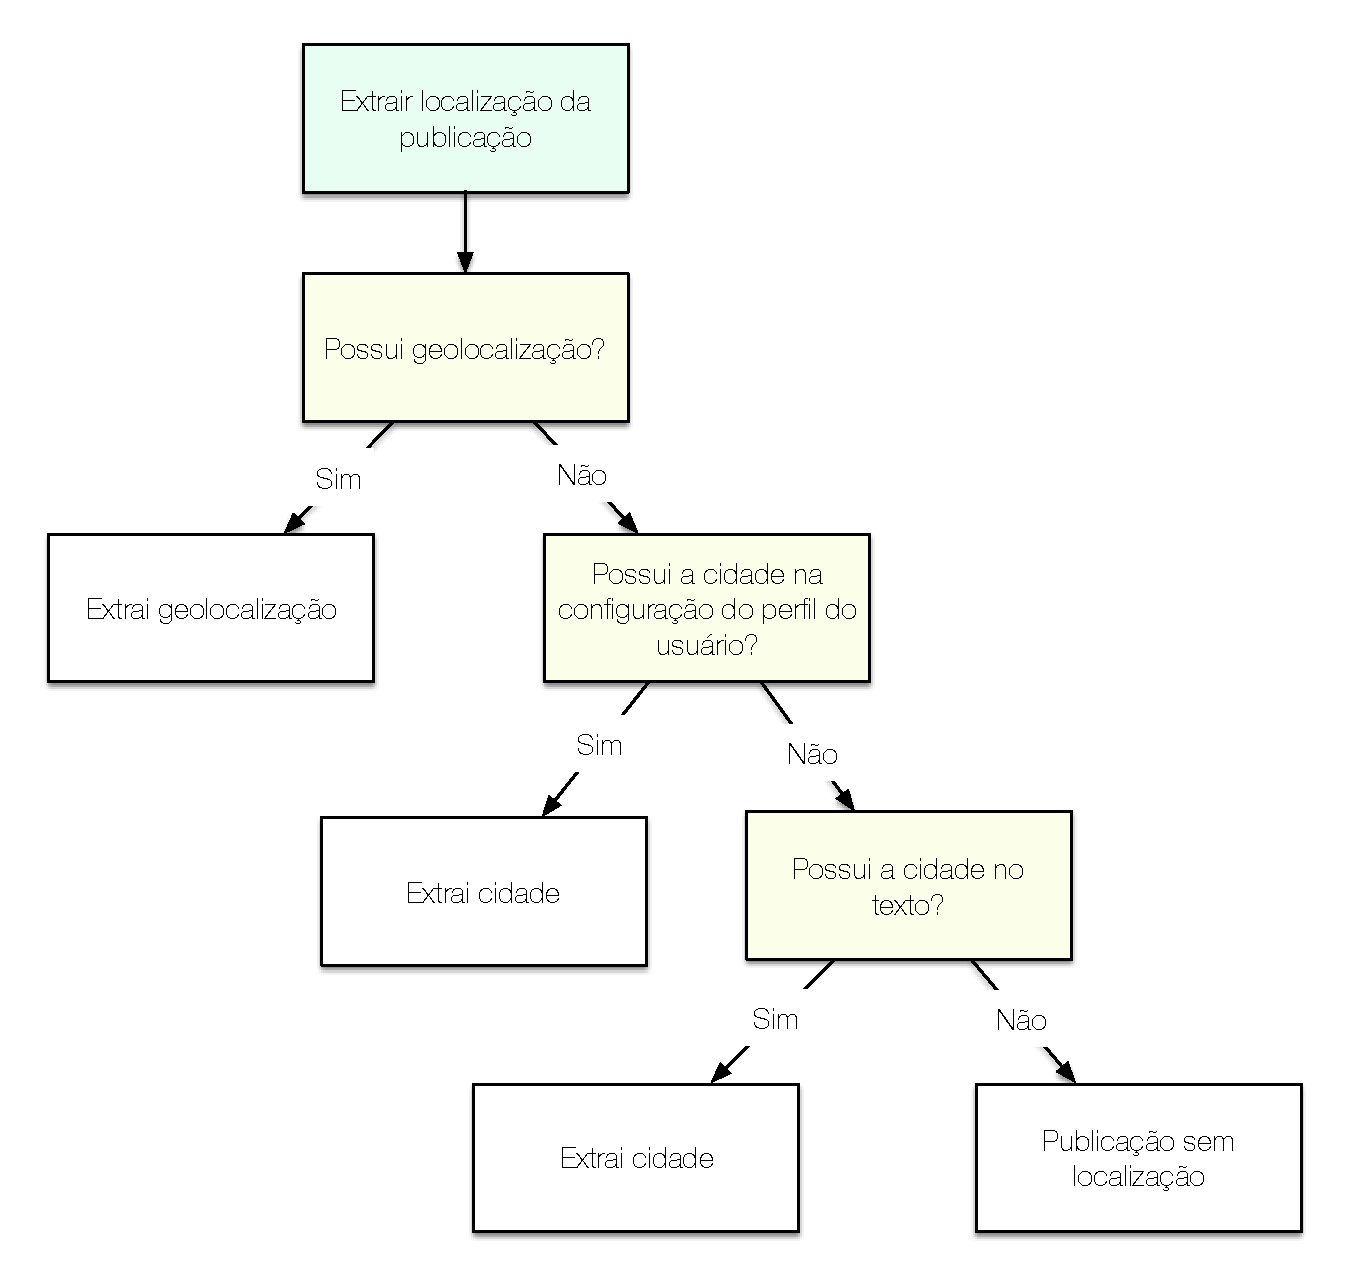
\includegraphics[width=1.0\textwidth]{figuras/extracao-localizacao.eps}
  \caption{Árvore de decisão para extração da localização da publicação.}
  \end{center}
\end{figure}